\section{Theoretical Analysis}
\label{sec:analysis}

\subsection{Node analysis method ($t < 0$)}
\label{sec:node}

For the time interval $t < 0$, the voltage in the independent voltage source is constant, $v_S(t) = V_S$. As a consequence, to study the circuit in this interval, one can considere it has been on for such an amout of time  that the capacitor is fully charged, which implies that $I_c = 0$.

By analysing the circuit and using KCL and Ohm's Law, it is possible to perform a node analysis and to write an equation for each node as it follows:

\begin{equation}
  \begin{cases}
    (GND) & \frac{V_7}{R_6} + \frac{V_5}{R_4} + \frac{V_2-V_1}{R_1} = 0 \\
    (1) & V_1 = V_S \\
    (2) & -\frac{V_2-V_1}{R_1} - \frac{V_2-V_5}{R_3} + \frac{V_3-V_2}{R_2} = 0 \\
    (3) & I_b - \frac{V_3-V_2}{R_2} = 0 \\
    (5) & V_2-V_5 = V_b \\
    (6) & -I_b - \frac{V_6-V_5}{R_5} - I_c = 0 \\
    (7) & -\frac{V_7}{R_6} + \frac{V_8-V_7}{R_7} = 0 \\
    (8) & V_5-V_8 = V_d
  \end{cases}
\end{equation}

Rearranging these equations and employing the relations $I_b = K_bV_b$ and $V_d = K_dI_d$, it is possible to write the following matrix system:

\begin{equation}
  \begin{bmatrix}
    -\frac{1}{R_1} & \frac{1}{R_1} & 0 & \frac{1}{R_4} & 0 & \frac{1}{R_6} & 0 \\
    1 & 0 & 0 & 0 & 0 & 0 & 0 \\
    \frac{1}{R_1} & -\frac{1}{R_1}-\frac{1}{R_2}-\frac{1}{R_3} & \frac{1}{R_2} & \frac{1}{R_3} & 0 & 0 & 0 \\
    0 & K_b + \frac{1}{R_2} & -\frac{1}{R_2} & -K_b & 0 & 0 & 0 \\
    0 & -K_b & 0 & K_b+\frac{1}{R_5} & -\frac{1}{R_5} & 0 & 0 \\
    0 & 0 & 0 & 0 & 0 & -\frac{1}{R_6}-\frac{1}{R_7} & \frac{1}{R_7} \\
    0 & 0 & 0 & 1 & 0 & \frac{K_d}{R_6} & -1     
  \end{bmatrix}
  \begin{bmatrix}
    V_1 \\
    V_2 \\
    V_3 \\
    V_5 \\
    V_6 \\
    V_7 \\
    V_8
  \end{bmatrix}
  =
  \begin{bmatrix}
    0 \\
    V_S \\
    0 \\
    0 \\
    0 \\
    0 \\
    0
  \end{bmatrix}
\end{equation}

Using {\bf Octave}, it was possible to use the matrix to compute the voltages in all nodes and the currents in all branches. These are presented in Table~\ref{node_res}. 

\begin{table}[H]
  \centering
  \begin{tabular}{|c|c|}
    \hline
        {\bf Name} & {\bf Value} \\
        \hline
        \hline
        $V_2\;(V)$ & $5.070727$ \\ 
\hline
$V_3\;(V)$ & $4.825468$ \\ 
\hline
$V_4\;(V)$ & $4.304579$ \\ 
\hline
$V_5\;(V)$ & $4.860091$ \\ 
\hline
$V_6\;(V)$ & $8.720760$ \\ 
\hline
$V_7\;(V)$ & $-2.939898$ \\ 
\hline
$V_8\;(V)$ & $-1.950198$ \\ 
\hline
$V_b\;(V)$ & $-0.034623$ \\ 
\hline
$I_b\;(V)$ & $-0.000251$ \\ 
\hline
$I_c\;(V)$ & $0.000969$ \\ 
\hline
$V_c\;(V)$ & $7.799989$ \\ 

        \hline
  \end{tabular}
  \caption{Theoretical results}
  \label{node_res}
\end{table}

\subsection{Capacitor behaviour}
\label{sec:Req}

In order to ascertain how the capacitor behaves, the equivalent resistor seen by it was determined. To do this, a tension source was added in lieu of the capacitor, and the response current of the remainder of the circuit was obtained, via node analysis methods.

For this procedure it was considered that $t=0\;s$, at which time the capacitor is fully charged, and so the voltage difference at it's terminals is known from \ref{sec:node} and constant (static analysis). At this time, it is also known that $V_s=0\;V$ - it is the exact time at which the source shifts from constant ($V_s$) to sinusoidal (null).

\begin{figure}[H]
  \centering
  \includegraphics[width=0.6\linewidth]{Req.pdf}
  \caption{Circuit}
  \label{Req_fig}
\end{figure}

There are seven unknowns, $V_1$, $V_2$, $V_3$, $V_5$, $V_6$, $V_7$ and $V_8$, and eight nodes. Given that the GND node does not constitute an unkown, it is not considered. One super-node equation is considered, regarding the eighth node, and it contais nodes 5, 6 and 8.

\begin{equation}
  \begin{cases}
    (1) & V_1=0 \\
    (2) & \frac{V_1-V_2}{R_1} + \frac{V_5-V_2}{R_3} + \frac{V_3-V_2}{R_2} = 0 \\
    (3) & I_b = \frac{(V_3-V_2)}{R_2} = 0 \\
    (5) & V_5-V_8 = V_d \\
    (6) & V_6-V_8 = V_x \\
    (7) & -\frac{V_7}{R_6} + \frac{V_8-V_7}{R_7} = 0 \\
    (8) & -\frac{V_5}{R_4}+\frac{V_2-V_5}{R_3}-I_b+\frac{V_7-V_8}{R_7} = 0
  \end{cases}
\end{equation}

Rearranging these equations and employing the relations $I_b = K_bV_b$ and $V_d = K_dI_d$, it is possible to write the following matrix system:

\begin{equation}
  \begin{bmatrix}
    1 & 0 & 0 & 0 & 0 & 0 & 0 \\
    \frac{1}{R_1} & -\frac{1}{R_1}-\frac{1}{R_2}-\frac{1}{R_3} & \frac{1}{R_2} & \frac{1}{R_3} & 0 & 0 & 0 \\
    0 & K_b + \frac{1}{R_2} & -\frac{1}{R_2} & -K_b & 0 & 0 & 0 \\
    0 & 0 & 0 & 1 & 0 & \frac{K_d}{R_6} & -1 \\
    0 & 0 & 0 & 0 & 1 & 0 & -1 \\
    0 & 0 & 0 & 0 & 0 & -\frac{1}{R_6}-\frac{1}{R_7} & \frac{1}{R_7} \\
    0 & \frac{1}{R_3}-K_b & 0 & 0 & -\frac{1}{R_4}-\frac{1}{R_3}+K_b & 0 & \frac{1}{R_7} & -\frac{1}{R_7}
  \end{bmatrix}
  \begin{bmatrix}
    V_1 \\
    V_2 \\
    V_3 \\
    V_5 \\
    V_6 \\
    V_7 \\
    V_8
  \end{bmatrix}
  =
  \begin{bmatrix}
    0 \\
    0 \\
    0 \\
    0 \\
    V_x \\
    0 \\
    0
  \end{bmatrix}
\end{equation}

The results obtained by solving this system using \textbf{Octave} are as follows:

\begin{table}[H]
  \centering
  \begin{tabular}{|c|c|}
    \hline
        {\bf Name} & {\bf Value} \\
        \hline
        \hline
        \input{../mat/nodeReq}
        \hline
  \end{tabular}
  \caption{Theoretical results}
\end{table}

By applying KCL to node 6, $I_x$ can be calculated:

\begin{equation}
  I_x = I_b - \frac{V_5-V_6}{R_5} = K_b \cdot (V_2-V_5) - \frac{V_5-V_6}{R_5} 
\end{equation}

$R_{eq}$ is then obtained from Ohm's Law:

\begin{equation}
  R_{eq} = \frac{V_x}{I_x}
\end{equation}

\begin{table}[H]
  \centering
  \begin{tabular}{|c|c|}
    \hline
        {\bf Name} & {\bf Value} \\
        \hline
        \hline
        \input{../mat/nodeReq2}
        \hline
  \end{tabular}
  \caption{Theoretical results}
\end{table}

As expected, the current value $I_x$ is negative, thus making $P_x$ negative (the current going through $V_x$ is $-I_x$): the voltage source supplies energy to the circuit. We can then reduce the capacitor's behaviour to:

\begin{figure}[H]
  \centering
  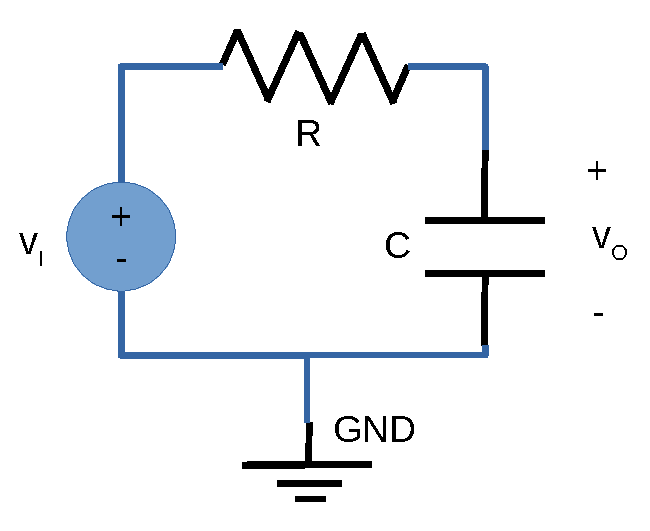
\includegraphics[width=0.6\linewidth]{rc.pdf}
  \caption{Equivalent RC circuit}
  \label{rc_fig}
\end{figure}

In order to confirm the above results do not depend on the potencial difference at the capacitor terminals ($V$), it was also solved using a symbolic package in \textbf{Octave}, which determined:

\begin{table}[H]
  \centering
  \begin{tabular}{|c|c|}
    \hline
        {\bf Name} & {\bf Value} \\
        \hline
        \hline
        \input{../mat/nodeReqb}
        \hline
  \end{tabular}
  \caption{Symbolic solution}
  \label{sym}
\end{table}

It is then true that, no matter $v_c(t)=v_6(t)-v_8(t)$, as the capacitor discharges, all nodes have null potential except for $v_6(t)$.

\subsubsection{Natural solution}

The natural solution of the capacitor behaviour is obtained by considering $v_x(t\geq0)=0$ and $v(0)=V_x$, where $v$ is as depicted in Figure~\ref{rc_fig}. From Table \ref{sym}, we can safely say that $v_8(t)=0\;V$ and $v(t)=v_6(t)\;V$ for the natural response (that is, with $v_s=0\;V$). It is known that:

\begin{equation}
  \begin{cases}
    KVL: & v(t) + R_{eq} \cdot i(t) = 0 \\
    Capacitor: & i(t) = C \cdot \frac{dv(t)}{dt}
  \end{cases}
  \label{sis}
\end{equation}

A first order linear equation arises from \ref{sis}, which can be readily solved:

\begin{equation}
  RC \cdot \frac{dv(t)}{dt} + v(t) = 0 \Rightarrow v(t) = Ae^{-\frac{t}{RC}}
\end{equation}

Applying the initial condition:

\begin{equation}
  v(0) = A = V_x
\end{equation}

The natural solution is:

\begin{equation}
  \label{nat_sol} v(t) =
  \begin{cases}
    V_x & \mbox{if } t \leq 0 \\
    V_xe^{-\frac{t}{RC}} & \mbox{if } t > 0
  \end{cases}
\end{equation}

\begin{figure}[H]
  \centering
  \includegraphics[width=0.8\linewidth]{natural.eps}
  \caption{Natural response}
  \label{fig:nat}
\end{figure}

\subsubsection{Forced solution}

The forced behaviour of the capacitor is obtained for $t > 0$, during which time $v_s(t)$ is a sine wave. To study this,  another node analysis was performed. The equations used were the same as the ones already presented in Section~\ref{sec:node}, but in this case, $I_c$ is not zero. For this situation $I_c = \frac{V_6-V_8}{Z}$, where $Z = \frac{1}{jwC}$ is the impedance of the capacitor, which has capacitance C. $w = 2\pi f$ is the radial frequency of the signal of $v_s(t) = \sin(wt) = \cos(wt-\frac{\pi}{2})$. This sinusoidal excitation will induce a sinusoidal forced solution with the same frequency for the components of the circuit.

\begin{figure}[H]
  \centering
  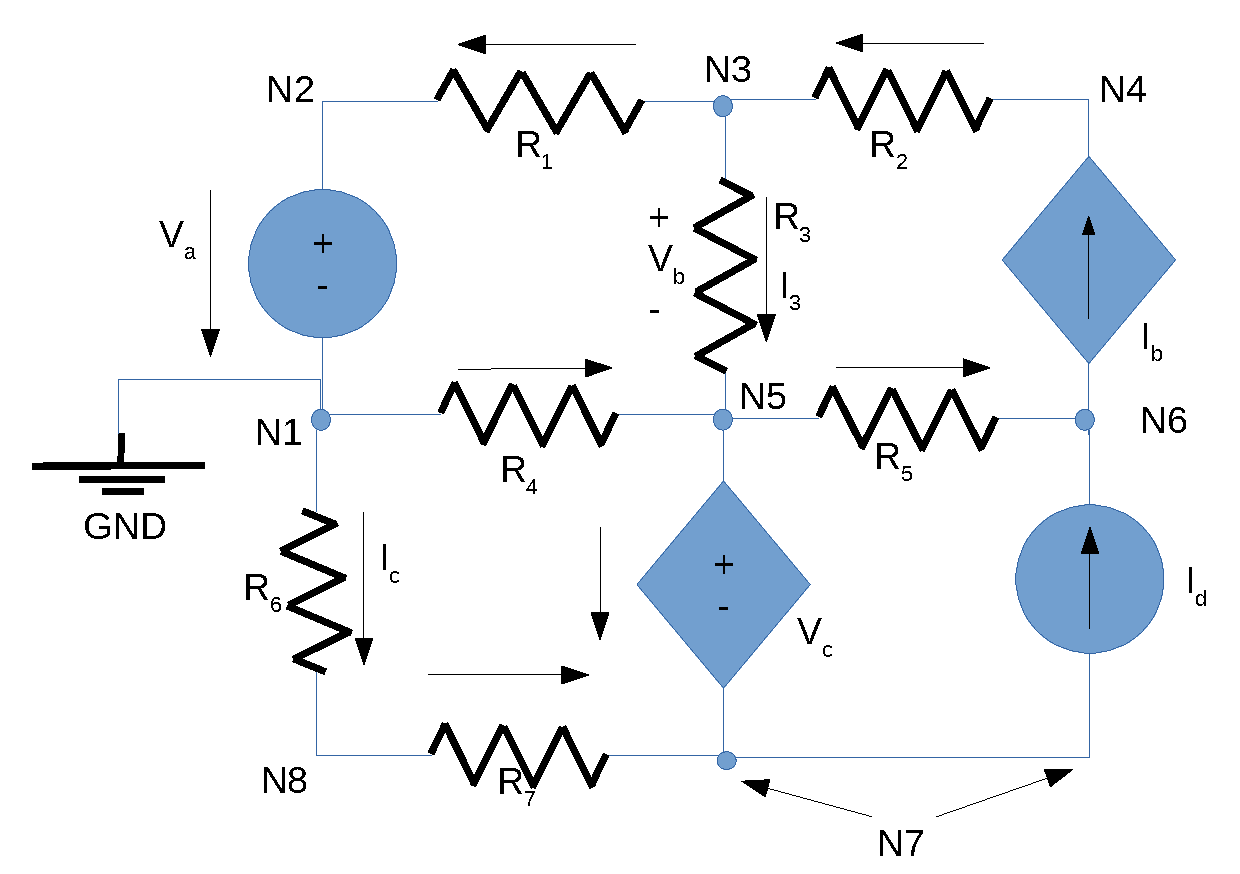
\includegraphics[width=0.6\linewidth]{node.pdf}
  \caption{Circuit}
  \label{node_fig}
\end{figure}

Consequently, the voltages in the nodes for the forced solution will have the form of $V_i\cos(wt-\phi_i)$. It is possible to compute the voltages in the nodes by representing these voltages as phasors (that is, complex numbers that return the amplitude and phase difference of the response). Solving the matrix below, with {\bf Octave}, gives the values of the phasors, that are in table \ref{forced_res}. The module of these complex numbers gives the amplitude $V_i$ and their angle is the phase delay $\phi_i$.

So, using the results of \ref{forcedamplitudes_res}, it is possible to conclude that

\begin{equation}
  \input{../mat/forced6}
\end{equation}

%The phase delay with respect to the source is equal to $\frac{\pi}{2}-\phi_i$.

\begin{equation}
  \begin{bmatrix}
    -\frac{1}{R_1} & \frac{1}{R_1} & 0 & \frac{1}{R_4} & 0 & \frac{1}{R_6} & 0 \\
    1 & 0 & 0 & 0 & 0 & 0 & 0 \\
    \frac{1}{R_1} & -\frac{1}{R_1}-\frac{1}{R_2}-\frac{1}{R_3} & \frac{1}{R_2} & \frac{1}{R_3} & 0 & 0 & 0 \\
    0 & K_b + \frac{1}{R_2} & -\frac{1}{R_2} & -K_b & 0 & 0 & 0 \\
    0 & -K_b & 0 & K_b+\frac{1}{R_5} & -\frac{1}{R_5}-jwC & 0 & jwC \\
    0 & 0 & 0 & 0 & 0 & -\frac{1}{R_6}-\frac{1}{R_7} & \frac{1}{R_7} \\
    0 & 0 & 0 & 1 & 0 & \frac{K_d}{R_6} & -1     
  \end{bmatrix}
  \begin{bmatrix}
    V_1 \\
    V_2 \\
    V_3 \\
    V_5 \\
    V_6 \\
    V_7 \\
    V_8
  \end{bmatrix}
  =
  \begin{bmatrix}
    0 \\
    V_S \\
    0 \\
    0 \\
    0 \\
    0 \\
    0
  \end{bmatrix}
  \label{pha}
\end{equation}

\begin{table}[H]
  \centering
  \begin{tabular}{|c|c|}
    \hline
        {\bf Name} & {\bf Value} \\
        \hline
        \hline
        \input{../mat/forced}
        \hline
  \end{tabular}
  \caption{Theoretical results}
  \label{forced_res}
\end{table}

\begin{table}[H]
  \centering
  \begin{tabular}{|c|c|c|}
    \hline
        {\bf Name} & {\bf Amplitude} & {\bf Phase (rad)} \\
        \hline
        \hline
        \input{../mat/forced2}
        \hline
  \end{tabular}
  \caption{Theoretical results}
  \label{forcedamplitudes_res}
\end{table}

\subsubsection{Final solution}

The final solution can be obtained by superimposing the natural and forced solutions.

\begin{figure}[H]
  \centering
  \includegraphics[width=0.8\linewidth]{total.eps}
  \caption{Total response and source signal (for comparison)}
  \label{fig:tot}
\end{figure}

\subsection{Frequency response}

By solving the system \ref{pha} and considering $f$ an unknown ($w=2\pi f$), using a symbolic package in \textbf{Octave}, it is possible to determine $v_6(f)$ and $v_8(f)$, where both are complex functions of a real variable. To better characterize the behaviour of the capacitor, the following graphs were made:

\begin{figure}[H]
  \centering
  \includegraphics[width=0.8\textwidth]{freq_response_mag.eps}
  \caption{Magnitude frequency response}
  \label{freq_resp_mag}
\end{figure}

\begin{figure}[H]
  \centering
  \includegraphics[width=0.8\textwidth]{freq_response_phi.eps}
  \caption{Phase frequency response}
  \label{freq_resp_pha}
\end{figure}

In order to ensure ease of comparison, in the latter graph it is not considered $\phi$ as calculated theoretically. This analysis considered a signal of the form $\cos(\omega t - \phi)$, while the simulation considers a signal of the form $\sin(\omega t + \phi')$. It is easy to determine that $\phi' = \frac{\pi}{2} - \phi$ in radians, or $\phi' = 90 - \phi$ in degrees. The graph in Figure~\ref{freq_resp_pha} then portrays $\phi'$, as does Figure~\ref{freq_resp_pha_sim}.
